\insertdesignoverview{Jewel Hitter}
{Create a unique design that quickly knocks off the jewel to save time for scoring multiple glyphs in autonomous} % Goals of the mechanism
{front_jewel.JPG}% CAD Image
{side_unloaded.JPG}% Build Image
{1/8" Steel Rod, Aluminum, 1/8" Black Tubing, String}% Materials ex. 0.25" MDF, Aluminum, etc
{Lathe work, Welding, Knot Tying}% Manufacturing Processes ex. Laser Cut, 3D print, etc.

\subsection*{How it Works}
There are two poles at the bottom of the robot, connecting the two drive train sides together. Dircetly, above them are two additional poles.
A hollow tube contains a pulley at the back and a pin that goes through the front of the tube. A thin pole has a string attached to it that is redirected to the tube above with two pulleys. The string in the top tube is wrapped around two additional pulleys within the tube, resulting in a 3 to 1 reduction. The string then connects to surgical tubing fixed at one end of the top tube.

To load the shooter, simply pull out the shooter pole and shove it back in on the opposite side of the pin, stretching the surgical tubing. THe front of the shooter is held in by a servo. Then the servo frees the jewel hitter, causing it to shoot out, go on the opposite side of the pin, and retract in one swift motion. 


\begin{figure}[htp]
\centering
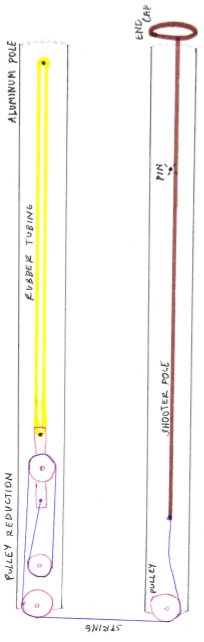
\includegraphics[width=.25\linewidth, angle = 270]{Design_Overview/jewel_hitter_diagram.PNG}
\caption{Diagram of jewel hitter}
\label{fig:Jewel_Dig}
\end{figure}


\begin{figure}[htp]
\centering
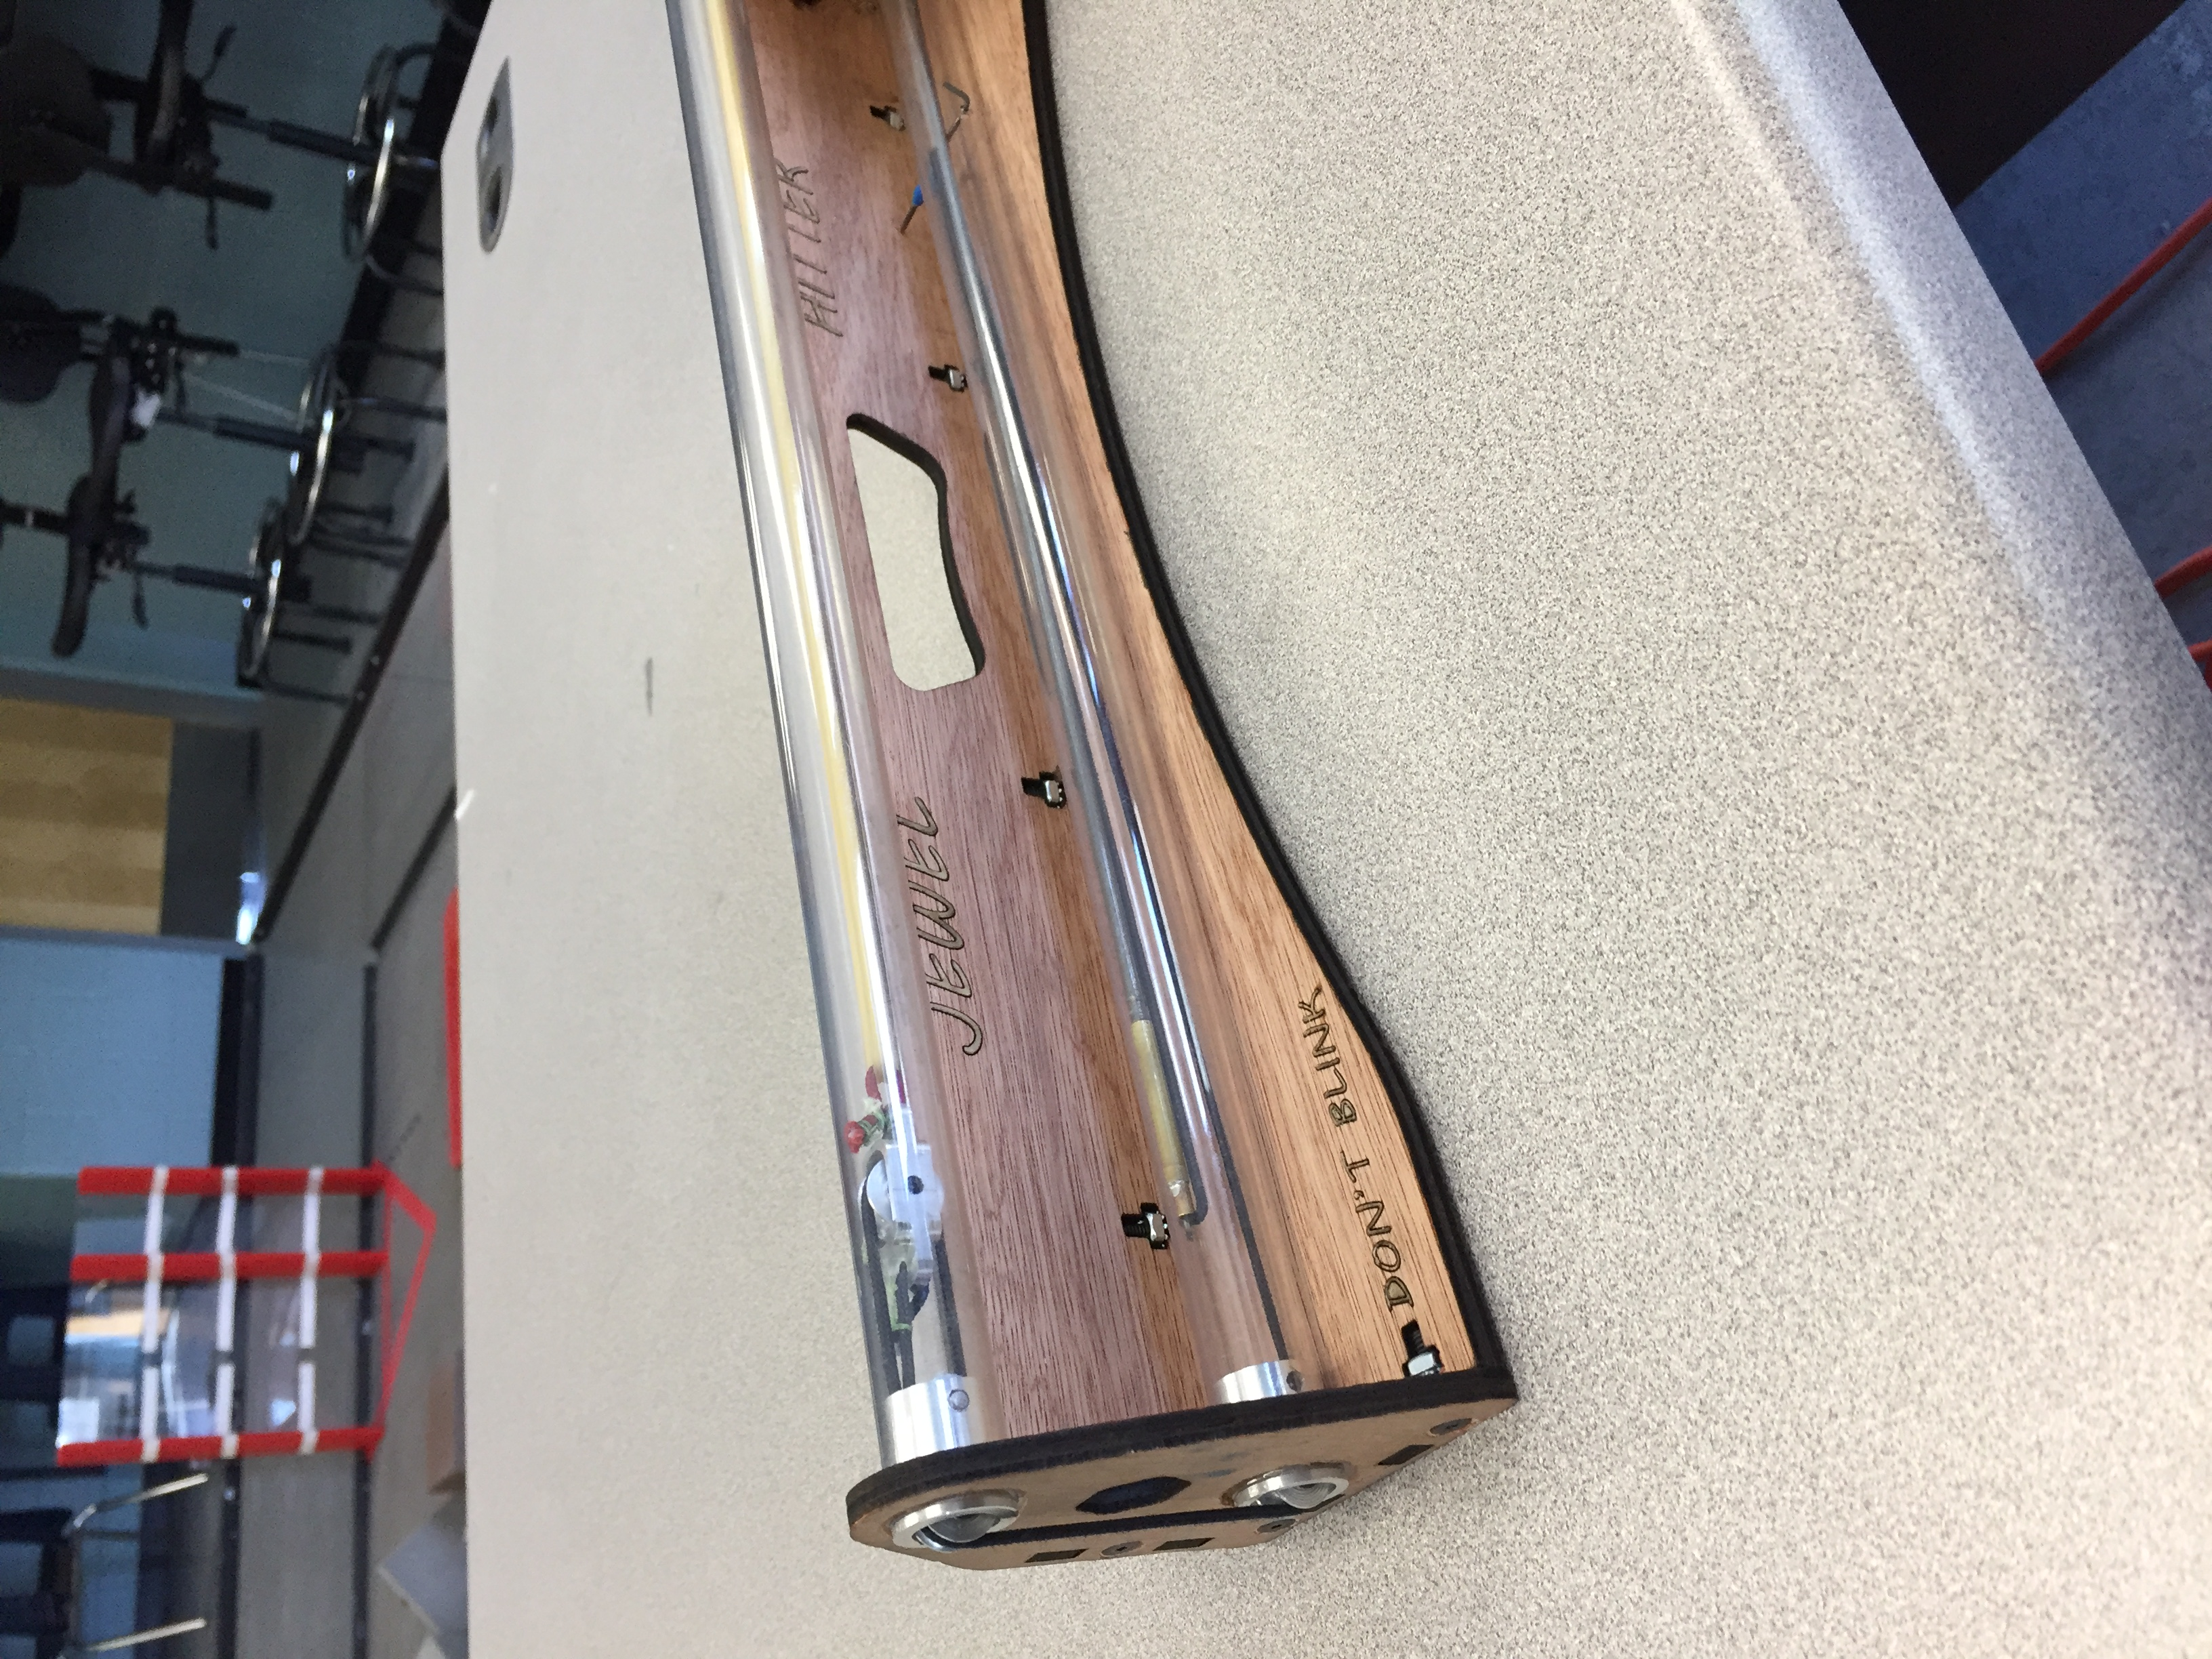
\includegraphics[width=.4\linewidth, angle =270]{Design_Overview/loaded_side_jewel.JPG}
\caption{Inside look at the jewel hitter in its loaded state}
\label{fig:inside}
\end{figure}



\subsection*{Iterations}
Initially, the caps and pulley of the jewel hitter were 3D printed. We found that we couldnt get the high resolution and strength we needed, so we decided to manufacture these parts out of aluminum. 

We also thought we could house the rubber band and shooter pole in one aluminum tube. This overcroweded the tube, forcing us to use a thin and weak rubber band that would always break. 

\subsection*{Sensors and Control} 
We have a PIXY camera that returns coordinates of color blobs. It detects the order of the jewels on the stand.

\begin{figure}[htp]
\centering
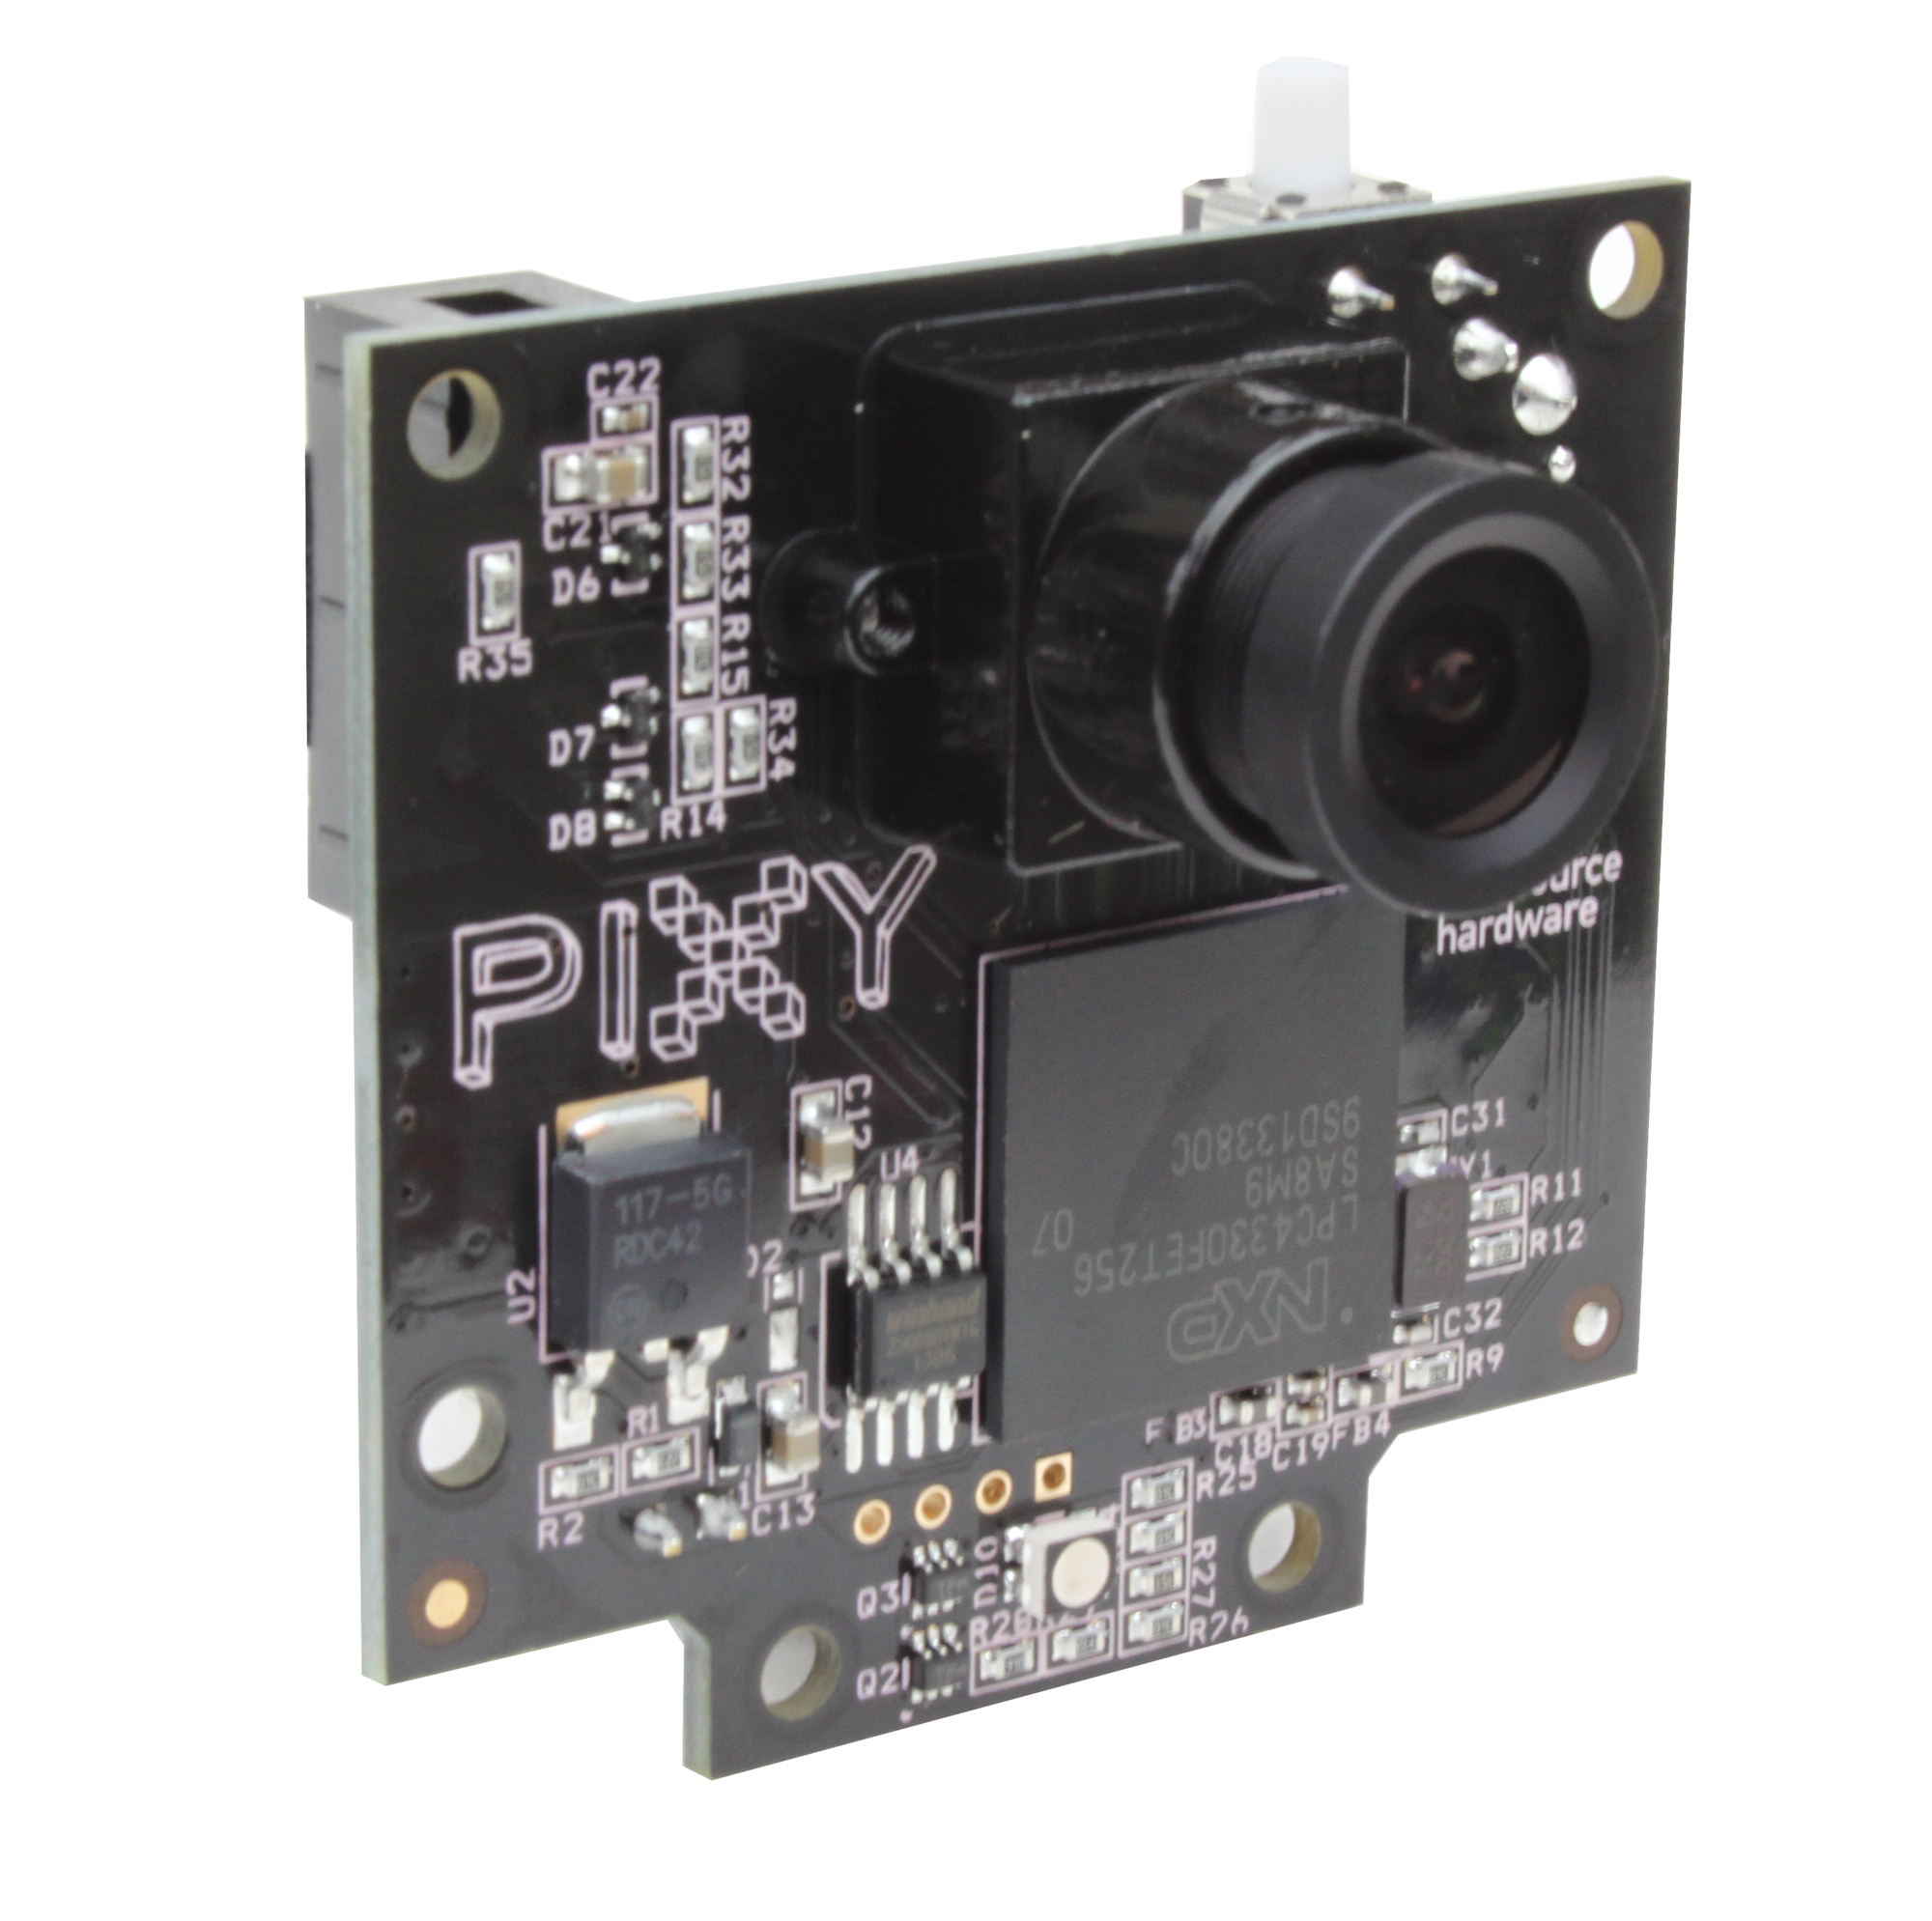
\includegraphics[width=.5\linewidth]{Design_Overview/pixy_camera.jpg}
\caption{PIXY Camera for detecting the jewels}
\label{fig:pixy_cam}
\end{figure}